\section{Diseño}

Para el modelado de este proyecto se buscó utilizar prácticas recomendadas y algunos de los patrones vistos con el fin de obtener un modelo cerrado para la modificación pero abierto para la extensión, minimizar la repetición de código, crear buenas abstracciones y permitir variaciones de comportamiento eficientes en tiempo de ejecución. Es importante recalcar que, tal como se explicó en los comentarios de la experiencia con $Scrum$, el modelado no siempre precedió a la implementación, sino que ambos procesos se vieron intercalados y retroalimentados a medida que se avanzaban con distintas $user\ stories$ y se realizaban puestas en común entre el grupo. En esta sección presentamos la visión final del diseño con aquellas soluciones que concluímos eran las más adecuadas, aunque se incluyen comentarios respecto a qué ideas se descartaron o modificaron cuando resulte relevante el contraste.

\subsection{Idea general}

En esta primera etapa del desarrollo, la HOP regula los cultivos de dos maneras: mediante un monitoreo pautado por un plan maestro y por medio de suministros arbitrarios programados en un plan de suministros. Esta interacción con el mundo real está dada, en principio, por dos vías: la recepción de datos mediante sensores y la aplicación de suministros mediante actuadores. Existe una tercera vía de comunicación con el exterior, la cual importa para la toma de decisiones, e involucra envío de mensajes a terceros (se descuenta la interacción por pantalla para mostrar información general).\\
\indent En el caso del plan maestro, éste define para una serie de estadíos fenológicos el estado de suelo deseado (humedad, temperatura, ph). El de suministros, en cambio, debe proveer la programación de insumos para una jornada, lo que incluye una lista de actuadores por cada hora del día y una medida a suministrar para cada uno. Tanto el monitoreo como el suministro arbitrario está a su vez regulado por supervisores que, según su tipo, pedirán información a sensores y en base a esto desencadenarán o no una cadena de responsabilidades hasta que se llegue a una decisión respecto de si suministrar el insumo adecuado o no.

\subsection{Plan Maestro: Estados y Magnitudes}

Antes de comenzar a hablar de las componentes más ricas del diseño es necesario detallar brevemente la parte más sencilla del mismo, que tiene que ver con la representación de parte de la información que se necesita conocer o decir sobre la realidad. Por un lado, se cuenta con la clase concreta \textsl{Medida}, que poseee como colaboradores internos una cantidad y una constante que da cuenta de la unidad correspondiente. Esto permite modelar tanto la información (medición) que se obtiene de los sensores así como también cuantificar el suministro de insumos (esto permitirá representar distintas magnitudes según se definan nuevas unidades, tanto para la incorporación de otros sensores como para el suministro de nuevos insumos). Luego, \textsl{EstadoSuelo} se compone de tres datos: medidas de temperatura, ph y humedad. Algo parecido sucede con \textsl{EstadoMeteorológico}, que a diferencia de la primera - que se utiliza para administrar el suelo en estadíos fenológicos - se utiliza para modelar el clima. Finalmente, la clase \textsl{Etapa} sólo se utiliza para encapsular nombres de estadíos fenológicos, que se definen de manera global para toda la HOP.\\
\indent A partir de estas representaciones básicas entra en juego la clase contenedora \textsl{PlanMaestro}, que posee como variable de instancia un \textsl{Diccionario}\verb|<|\textsl{Etapa, EstadoSuelo}\verb|>| mediante el cual permite definir las etapas fenológicas a monitorear y los valores esperados del estado del suelo. Notar que este modelo permite agregar estados o modificar los existentes dinámicamente (aunque esto último tendrá un impacto como se verá luego).\\
\indent En una los albores de la planificación y posterior modelado, el Plan Maestro tenía más responsabilidades que simplemente dictar cuál es el estado ideal de los cultivos: debía determinar también acciones a llevar adelante, información del estado, comunicación con la central meteorológica, etc. Esta idea desembocaba en un objeto que centralizaban gran parte de la lógica de resolución del problema y, claramente, tenían varios ejes de cambio y mucho acoplamiento, lo cual se fue decantando de manera natural a medida que se iteraba sobre el modelo con nuevas ideas y patrones de diseño.

\subsection{Sensores, Actuadores y Responsables}
Comenzamos con una de las partes fundamentales del sistema que es la medición de los sensores y la consecuente ejecución de un actuador. \newline

 
En un comienzo encaramos el diseño de esta parte del sistema pensando a los distintos sensores como observadores del Plan Maestro. Esta idea fue luego descartada por no tener ninguna razón para sacarle provecho al patrón observer y porque convertía al Plan Maestro en un objeto con demasiadas responsabilidades (conocer los sensores, sus estados, los estadíos de la planta, etc).

A su vez, pensamos diseñar los distintos planes de suministro con un strategy pattern con la idea de que sean extensibles esos planes, pero finalmente concluímos que no era necesario.\newline


 
Otro error común que tuvimos a la hora de pensar el diseño fue el de discriminar parte del dominio de una mala manera. Por ejemplo, separando entre actuadores regulables y actuadores suministrables. Esto vino de la mano de pensar la modernización de los recursos como recursos suministrables y regulables. Esta idea también fue eliminada por generar una buena cantidad de objetos cuya escénica era la misma pero estaban separados, generando así que al momento de modificar código tengamos que reemplazarlo en varios lugares al mismo tiempo.\newline

 
En la figura 1 puede verse el diagrama de clases elegido luego de todas estas discusiones y reformas.

\begin{figure}[h!]
  \centering
  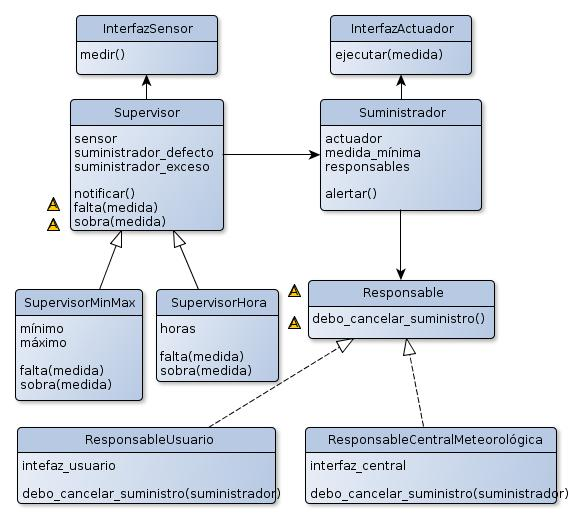
\includegraphics[width=0.8\textwidth]{./imagenes/clases2.jpg}
  \caption{Diagrama de Clases}
  \label{fig:sec_sum1}
\end{figure}


\newpage Vamos a profundizar en cada objeto:

\begin{itemize}
\item \textbf{InterfazSensor:} Este objeto tiene como colaborador interno a un sensor (de humedad, suelo, etc) y nos brinda una interfaz sencilla para comunicarnos y obtener la medición correspondiente a ese sensor.

\item \textbf{InterfazActuador:} Al igual que para los sensores, este objeto nos brinda una interfaz sencilla para interactuar con un actuador, que es colaborador interno del objeto InterfazActuador. Ambas soluciones pueden interpretarse como un adapter pattern.

\item \textbf{Supervisor:} Esta es una clase de la cual heredan los distintos supervisores que vayan a usarse. Un supervisor se encarga de interpretar las mediciones y alertar en caso de que sea necesario realizar una acción. Para esto cuenta con 2 colaboradores: un suministrador por falta y un suministrador por exceso. Es el primer eslabón en la cadena de decisión.

\item \textbf{Suministrador:} Es el encargado de recibir una alerta por parte del supervisor y tomar la decisión final de ejecutar o no, la acción requerida. Para esto cuenta con una colección de responsables, que son objetos capaces de responder a la consulta de si efectivizar o no la acción. Por ejemplo, un responsable es el usuario (que se le consulta a través de una interfaz), otro es el responsable de la Central Meteorológica. De esta forma, en una posible versión futura, el sistema permite la integración de nuevos módulos de consulta para automatizar las decisiones.

\item \textbf{Responsable:} Como se vio recién, esta es una interfaz que la implementarán aquellos objetos que cumplan el rol de responder ante la consulta de si realizar o no una tarea. 
\end{itemize}
Para entender mejor el funcionamiento, más adelante se detalla un diagram de secuencia correspondiente a una nueva medición de humedad.


\subsection{Timer}
Una vez que concluimos en utilizar ese diseño para los sensores y actuadores del sistema, nos encontramos con la dificultad de pensar quien tomará el rol de avisar a los distintos supervisores que es momento de supervisar. La solución apareció bastante rápido y se trata de un timer y un observer pattern.

El timer es un objeto observable y los supervisores implementan la interfaz de observadores. De esta forma, los distintos supervisores se registran con el timer y este les avisa cada cierta cantidad de tiempo que es momento de supervisar.

Esta solución nos permite variar la cantidad de supervisores en caso de que se aumenten los sensores que se utilizan.

\textbf{ACA ALGÚN DIAGRAMA}

\subsection{Coordinador}
Los parámetros utilizados para decidir si una medición provoca o no una alerta van a variar según la etapa en la que se encuentre el cultivo. Esto provocará que los supervisores que se encargan de tomar esas decisiones tengan que cambiar su funcionamiento. Sin embargo, el resto de los objetos no deben verse afectados en absoluto.

Por esta razón, decidimos agregar al diseño un coordinador, encargado de mantener la información necesaria para modificar los supervisores que se encuentran operando. 

Este coordinador mantiene la información del Plan Maestro y los distintos Planes de Suministro por etapa, así como los actuadores y acciones disponibles.

\begin{figure}[h!]
  \centering
  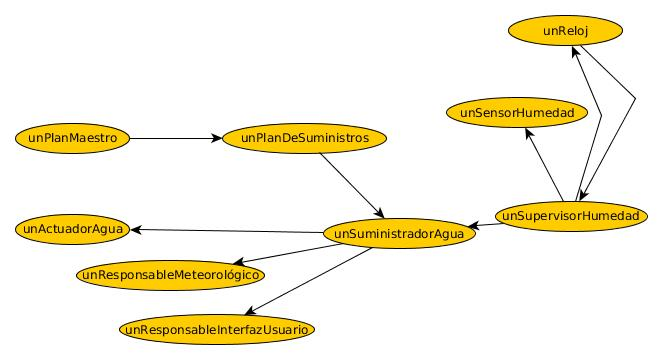
\includegraphics[width=1\textwidth]{./imagenes/objetosCoordinador.jpg}
  \caption{Diagrama de colaboración}
  \label{fig:sec_sum1}
\end{figure}


\subsection{Estados y Mediciones}
Tanto para el estado del suelo como el estado meteorológico, contamos con sus objetos correspondientes que tienen la información humedad, ph y temperatura (en el caso del suelo), y humedad, temperatura y luz (en el otro caso).

Para ambos estados, las mediciones están representadas por el objeto \textit{Medida} que  tiene una cantidad y una unidad de medida.

\textbf{ACA ALGÚN DIAGRAMA}



\subsection{Situación: nueva medición de humedad}
Vamos a tomar un caso para ejemplificar el comportamiento del sistema al recibir una nueva medición y su consecuente resolución.

\begin{figure}[h!]
  \centering
  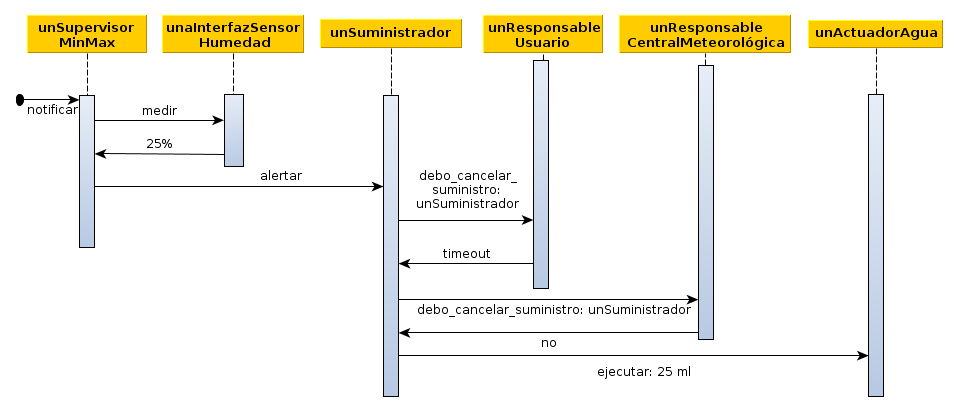
\includegraphics[width=1\textwidth]{./imagenes/secuencia_suministro1.png}
  \caption{Diagrama de secuencia suministro}
  \label{fig:sec_sum1}
\end{figure}

A medida que transcurre el tiempo, el temporizador envía el mensaje de actualización a los distintos supervisores. 
Los supervisores a su vez, se encargan de revisar el estado de los distintos sensores para decidir si alertar o no en caso de un estado no deseado.
En este caso, espera la respuesta de la interfaz de humedad. Como vimos antes, las interfaces de sensores cumplen el rol de responder los mensajes de pedido de actualización de estado. 
El supervisor se encarga de reconocer en los datos situaciones que deben alertarse. Es así el caso del ejemplo, donde luego de recibir la actualización alerta al suministrador correspondiente.

El suministrador, previo a ejecutar la acción para suplir la alerta, colabora con la interfaz de usuario para permitir la cancelación de la acción. En caso de no haber respuesta (timeout) consulta a un responsable secundario (en este caso, el coordinador meteorológico) que nuevamente tiene la posibilidad de cancelar la acción.

Si algún responsable responde al mensaje, (es decir, no hay timeout) el suministrador actúa según la respuesta. En caso de recibir timeout de todos los responsables, decide efectuar la acción.

La acción la realiza finalmente, el actuador correspondiente.
